\chapter{The shallow water equations}\label{ch:theory}
In this chapter we will derive the shallow water equations (SWE) in conservative form, and present the equations in vector form and in integral form for 1D and 2D in cartesian coordinates.
We will also derive the SWE in spherical coordinates, which is relevant for geophysical applications, such as simulating water flow on the surface of the Earth.
To solve the SWE, we will present the numerical method, called the Finite Volume Method (FVM) including the Riemann problem.
Lastly, we will dive into the theory behind the data-driven methods, i.e., the neural networks and fourier neural operators.

\section{Notation}
Before deriving the shallow water equations (SWE), we will introduce the notation that will be used throughout this report.
In both the 1D and 2D cases of SWE, we use cartesian coordinates $(x, y, z)$ with time denoted by $t$.
Given that linear algebra is a fundamental tool used in this report, we first establish the relevant notation.
Lowercase bold letters represent vectors, while uppercase bold letters represent matrices.
For instance, $\mathbf{a}$ is a vector of size $1 \times r, r \in \mathbb{R}$, and $\mathbf{A}$ is a matrix of size $m \times n, m,n \in \mathbb{R}$.
The identity matrix, denoted by $\mathbf{I}$, is a square matrix with ones along the diagonal and zeros elsewhere.
For example, the $3 \times 3$ identity matrix is given by:
\begin{align*}
    \mathbf{I} = \begin{bmatrix}
        1 & 0 & 0 \\
        0 & 1 & 0 \\
        0 & 0 & 1
    \end{bmatrix}.
\end{align*}
We use the following notation for partial derivatives:
\begin{align*}
   f_x =  \frac{\partial f}{\partial x}, \quad f_y = \frac{\partial f}{\partial y}, \quad f_z = \frac{\partial f}{\partial z}.
\end{align*}
The gradient operator, denoted by $\nabla$, gives the gradient of a scalar function $f$ as a vector:
\begin{align*}
    \nabla f = \begin{bmatrix}
        \frac{\partial f}{\partial x} &
        \frac{\partial f}{\partial y} &
        \frac{\partial f}{\partial z}
    \end{bmatrix}.
\end{align*}
Given two vectors $\mathbf{a} = \begin{bmatrix}
    a_1 & a_2 & a_3
\end{bmatrix}^\top $ and $\mathbf{b} = \begin{bmatrix}
    b_1 & b_2 & b_3
\end{bmatrix}^\top$, the dot product of $\mathbf{a}$ and $\mathbf{b}$ is given by:
\begin{align*}
    \mathbf{a} \cdot \mathbf{b} = a_1 b_1 + a_2 b_2 + a_3 b_3.
\end{align*}
The dot product can also be written as a matrix product:
\begin{align*}
    \mathbf{a} \cdot \mathbf{b} = \mathbf{a}^\top \mathbf{b}.
\end{align*}
The divergence operator, represented as $\nabla \cdot $, gives the divergence of a vector $\mathbf{a}$ as:
\begin{align*}
    \nabla \cdot \mathbf{a} = \frac{\partial a_1}{\partial x} + \frac{\partial a_2}{\partial y} + \frac{\partial a_3}{\partial z} = {a_1}_x + {a_2}_y + {a_3}_z.
\end{align*}
The tensor product of two vectors $\mathbf{a}$ and $\mathbf{b}$, denoted as $\mathbf{a} \otimes \mathbf{b}$, is a matrix where each element is the product of the elements of $\mathbf{a}$ and $\mathbf{b}$, i.e.,
\begin{align*}
    \mathbf{a} \otimes \mathbf{b} = \begin{bmatrix}
        a_1 b_1 & a_1 b_2 & a_1 b_3 \\
        a_2 b_1 & a_2 b_2 & a_2 b_3 \\
        a_3 b_1 & a_3 b_2 & a_3 b_3
\end{bmatrix}.
\end{align*}






In this section we will derive the shallow water equations (SWE) in conservative form.

\section{Derivation of the SWE with conservative variables}
In this section we will derive the shallow water equations (SWE) in conservative form.
The Shallow Water Equations (SWE) are a set of hyperbolic partial differential equations that describe the motion of a fluid in a shallow layer of water.



The derivation follows four steps: First we consider the conservation laws for mass and momentum, and then we consider the boundary conditions for a free surface problem.
Afterwards we make some neccessary assumptions and finally we use the boundary conditions to integrate the conservation laws over depth.
The derivation follows the methods outlined in~\cite{Toro2001-Shock} and~\cite{Vreugdenhil1994}.


\subsubsection*{Conservation laws}
The SWE are derived from the conservation laws for mass and momentum, which are fundamental in fluid dynamics.
The conservation laws for mass and momentum can be expressed generally as follows (source: eq. (2.1) and (2.2) in~\cite{Toro2001-Shock}):
\begin{align}
    \rho_t + \nabla \cdot (\rho \mathbf{v}) = 0, \label{eq:mass_conservation} \\
    {(\rho \mathbf{v})}_t + \nabla \cdot (\rho \mathbf{v} \otimes \mathbf{v} + p \mathbf{I} - \mathbf{T}) = \rho \mathbf{g}, \label{eq:momentum_conservation}
\end{align}
where $\rho$ is the fluid density, $\mathbf{v} = \begin{bmatrix} u & v & w \end{bmatrix}^\top$ is the fluid velocity in the $x, y$ and $z-$direction respectively;
$p$ is the pressure, $\mathbf{I}$ is the identity matrix, and the vector $\mathbf{g} = \begin{bmatrix}
    g_1 & g_2 & g_3
\end{bmatrix}^\top$ represents body forces including gravity.
In these equations, the density $\rho$ and the pressure $p$ are dependent of $x, y, z$ and $t$, but later we will introduce some assumptions that simplify the equations.
The matrix $\mathbf{T}$ is the viscous stress tensor, given by
\begin{align*}
    \mathbf{T} = \begin{bmatrix}
        \tau_{xx} & \tau_{xy} & \tau_{xz} \\
        \tau_{yx} & \tau_{yy} & \tau_{yz} \\
        \tau_{zx} & \tau_{zy} & \tau_{zz}
    \end{bmatrix},
\end{align*}
which accounts for the viscous forces in the fluid.
However, in this project the viscous stress tensor $\mathbf{T}$ is neglected, since we assume the function $\tau(x,y,z)$ is constant.
The matrix $\mathbf{v} \otimes \mathbf{v}$ represents the tensor product of the velocity vector $\mathbf{v}$ with itself, i.e.,
\begin{align*}
    \mathbf{v} \otimes \mathbf{v} = \begin{bmatrix}
        u^2 & uv & uw \\
        vu & v^2 & vw \\
        wu & wv & w^2
    \end{bmatrix}.
\end{align*}
Note that $\mathbf{v} \otimes \mathbf{v} = \mathbf{v} \mathbf{v}^\top$.
Putting this together, we can rewrite the momentum equation~\eqref{eq:momentum_conservation} as
\begin{align}\label{eq:momentum_conservation_simplified}
    {(\rho \mathbf{v})}_t + \nabla \cdot (\rho \mathbf{v} \mathbf{v}^\top  + p \mathbf{I}) - \rho \mathbf{g} = 0.
\end{align}
In this project we consider incompressible fluids, meaning that the fluid density $\rho$ is independent of the pressure $p$.
We also assume that the fluid density only depends on temperature and salinity, and thus is independent of $t, x, y$ and $z$.
Additionally, we assume $\rho$ is nonzero.
Rewriting the mass conservation equation~\eqref{eq:mass_conservation} gives
\begin{align*}
    \rho_t + \rho(u_x + v_y + w_z) + u \rho_x + v \rho_y + w \rho_z = 0,
\end{align*}
using the given assumptions and the product rule for differentiation.
Hence we obtain
\begin{align}
    u_x + v_y + w_z = 0, \label{eq:mass_conservation_incompressible}
\end{align}
also referred to as the mass conservation equation.
Applying the divergence operator $\nabla \cdot$, the momentum conservation equation~\eqref{eq:momentum_conservation_simplified} can be written out as:
\begin{align}\label{eq:momentum_conservation_expanded}
    \rho_t \mathbf{v} + \rho \mathbf{v}_t + \rho \begin{bmatrix}
        {(u^2 + p)}_x + {(uv)}_y + {(uw)}_z \\
        {(vu)}_x + {(v^2 + p)}_y + {(vw)}_z \\
        {(wu)}_x + {(wv)}_y + {(w^2 + p)}_z 
    \end{bmatrix}
    - \rho \mathbf{g} = 0.
\end{align}
We neglect all body forces in $\mathbf{g}$, expect the gravitational force in the $z-$direction, i.e., $\mathbf{g} = \begin{bmatrix} 0 & 0 & -g \end{bmatrix}$, where $g$ is the gravity acceleration, which we assume to be constant.
Hence, by using the product rule in~\eqref{eq:momentum_conservation_expanded} and that $\rho_t = 0$ we obtain
\begin{align}\label{eq:momentum_conservation_expanded_final}
    \rho \begin{bmatrix}
        u_t \\ v_t \\ w_t
    \end{bmatrix}
    + \rho \begin{bmatrix}
        p_x + u u_x + v u_y + w u_z + u(u_x + v_y + w_z) \\
        p_y + u v_x + v v_y + w v_z + v(u_x + v_y + w_z) \\
        p_z + u w_x + v w_y + w w_z + w(u_x + v_y + w_z) 
    \end{bmatrix}
    - \rho \begin{bmatrix}
        0 \\ 0 \\ -g
    \end{bmatrix} = 0.
\end{align}
We apply~\eqref{eq:mass_conservation_incompressible} to~\eqref{eq:momentum_conservation_expanded_final} to remove some terms, we move the pressure terms to the right hand side, and we divide by $\rho$.
Putting it all together, the mass equation~\eqref{eq:mass_conservation} and the momentum equation~\eqref{eq:momentum_conservation_simplified}, split in $x, y$ and $z-$directions, simplify to 
\begin{equation}\label{eq:momentum_conservation_all}
    \left.
    \begin{aligned}
        u_x + v_y + w_z &= 0, \\
        u_t + u u_x + v u_y + w u_z &= - \frac{1}{\rho} p_x, \\
        v_t + u v_x + v v_y + w v_z &= - \frac{1}{\rho} p_y, \\
        w_t + u w_x + v w_y + w w_z &= - \frac{1}{\rho} p_z - g.
    \end{aligned}
    \right\}
\end{equation}


\subsubsection*{Boundary conditions}
In this project, we consider the flow of water with a free surface, meaning that the surface is not fixed and can move or change over time.
To solve the SWE, it is essential to impose boundary conditions at both the bottom of the water column and at the free surface.
We assumme the bottom $b$ is defined by a function
\begin{align*}
    z = b(x,y),
\end{align*}
meaning that the bottom is dependent on $x$ and $y$, but not on the time $t$.
Since the bottom is not moving over time, we refer to it as fixed.
The free surface is defined by 
\begin{align*}
    z = s(x,y,t) \equiv b(x,y) + h(x,y,t),
\end{align*}
where $h(x,y,t)$ is the water depth at time $t$.
The following illustration helps to visualize the setup:
\begin{figure}[H]
    \centering
    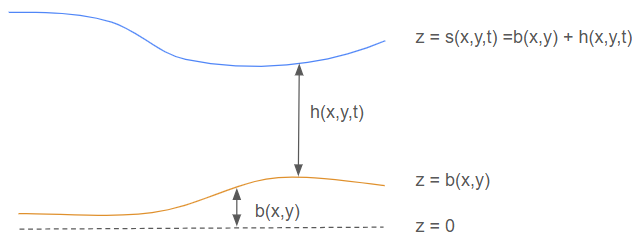
\includegraphics[width=0.6\textwidth]{figs/water-column-bc.png}
    \caption{Illustration of a water column with a free surface.}\label{fig:water_column_bc}
\end{figure}
We impose boundary conditions at the bottom and at the free surface, adressing both kinematic and dynamical conditions.
To describe the boundaries mathematically, we introduce a boundary function $\psi(x,y,z,t)$ that is zero on the boundaries:
\begin{align*}
    \psi(x,y,z,t) = 0.
\end{align*}
For the free surface, this boundary is given by
\begin{align}\label{eq:psi_free_surface}
    \psi|_{z = s} = z - s(x,y,t) = 0,
\end{align}
and for the bottom, it is described by
\begin{align}\label{eq:psi_bottom}
    \psi|_{z = b} = z - b(x,y) = 0.
\end{align}
In the kinematic condition, we assume that fluid particles on the boundary remain on the boundary over time.
Mathematically this is expressed as
\begin{align*}
    \frac{\text{d} }{\text{d} t} \psi(x,y,z,t) = 0.
\end{align*}
Recall, that $\frac{\partial \psi}{\partial t}$ is the partial derivative of $\psi$ with respect to $t$, while the total derivate $\frac{\text{d} \psi}{\text{d} t}$ accounts for both the direct change of $\psi$ with respect to $t$ and the changes due to the movement of the fluid in the $x, y$ and $z$ directions.
Hence, the total derivative of $\psi$ wrt. $t$ is given by
\begin{align*}
    \frac{\text{d} \psi}{\text{d} t} &= \frac{\partial \psi}{\partial t} + \frac{\text{d} x}{\text{d} t} \frac{\partial \psi}{\partial x} + \frac{\text{d} y}{\text{d} t}  \frac{\partial \psi}{\partial y} + \frac{\text{d} z}{\text{d} t}  \frac{\partial \psi}{\partial z}.
\end{align*}
We see that $\frac{\text{d}x}{\text{d}t}$ denotes the velocity in the $x-$direction, i.e., $u$, and correspondingly $\frac{\text{d}y}{\text{d}t}$ and $\frac{\text{d}x}{\text{d}t}$ denotes $v$ and $w$ respectively.
Thus, the kinematic condition is given by
\begin{align}\label{eq:kinematic_condition}
    \frac{\text{d} }{\text{d} t} \psi = \psi_t + u \psi_x + v \psi_y + w \psi_z = 0.
\end{align}
Applying this to the free surface by substituting~\eqref{eq:psi_free_surface} into the kinematic condition~\eqref{eq:kinematic_condition} yields
\begin{align}\label{eq:kinematic_condition_free_surface}
    (s_t + u s_x + v s_y - w)|_{z=s} = 0.
\end{align}
Similarly, for the bottom, substitung~\eqref{eq:psi_bottom} into the kinematic condition~\eqref{eq:kinematic_condition} gives
\begin{align}\label{eq:kinematic_condition_bottom}
    (u b_x + v b_y - w)|_{z=b} = 0.
\end{align}
The dynamical condition is related to the pressure distribution at the free surface.
We assume that the pressure at the free surface is equal to the pressure in the air above the surface, that is, the atmospheric pressure.
Since absolute pressure levels are irrelevant, as we are primarily concerned with pressure differences, we set the pressure at the free surface to zero.
This leads to the following expression for the pressure at the free surface:
\begin{align}\label{eq:pressure_free_surface}
    p(x,y,z,t)|_{z = s} = 0.
\end{align}
This condition, known as the dynamical condition, relates to the forces acting on the boundaries of the fluid.

\subsubsection*{Assumptions}
To derive the SWE it is neccessary to make some assumptions. 
The shallow water equations are an approximation to the full free-surface problem and result from the assumption that the vertical compononent of the acceleration is negligible.
Therefore, we begin by assuming that the vertical acceleration, represented by the total derivate of the vertical velocity component $w$ with respect to time, is negligible.
This assumption leads to the condition
\begin{align*}
    \frac{\text{d} w}{\text{d} t} = w_t + uw_x + vw_y + ww_z = 0.
\end{align*}
Applying $\frac{\text{d}w}{\text{d}t} = 0$ in the $z-$momentum conservation equation~\eqref{eq:momentum_conservation_all} simplifies it to
\begin{align*}
    p_z = -\rho g.
\end{align*}
By using properties of an integral, together with~\eqref{eq:pressure_free_surface} we get
\begin{align*}
    \int_{b(x,y)}^z - \rho g \text{ d}t + \int_z^{s(x,y,t)} - \rho g \text{ d}t = \int_{b(x,y)}^{s(x,y,t)} - \rho g \text{ d}t
    = p|_{z = s(x,y,t)} = 0.
\end{align*}
This implies that the pressure distribution follows
\begin{align}\label{eq:pressure_distribution}
    p = \int_{b(x,y)}^z - \rho g \text{ d}t = \int_z^{s(x,y,t)} \rho g \text{ d}t = \rho g (s - z),
\end{align}
where $s$ is the surface height.
Differentiating~\eqref{eq:pressure_distribution} with respect to $x$ and $y$ yields
\begin{align*}%\label{eq:pressure_distribution_x_y}
    p_x = \rho g s_x, \quad p_y = \rho g s_y.
\end{align*}
Substituting these expressions into the $x-$ and $y-$momentum conservation equations~\eqref{eq:momentum_conservation_all} leads to 
\begin{equation}\label{eq:momentum_conservation_xy_simplified}
    \left.
    \begin{aligned}
        u_t + u u_x + v u_y + w u_z &= -g s_x,  \\
        v_t + u v_x + v v_y + w v_z &= -g s_y,
    \end{aligned}
    \right\}
\end{equation}
which can be further simplified.
We realize that both $p_x$ and $p_y$ are independent of $z$, implying that $\frac{\text{d}u}{\text{d}t} $ and $\frac{\text{d}v}{\text{d}t} $are also independent of $z$.
Hence $u_z = v_z = 0$, implying that~\eqref{eq:momentum_conservation_xy_simplified} can be simplified to
\begin{equation}\label{eq:momentum_conservation_xy_final}
    \left.
    \begin{aligned}
        u_t + u u_x + v u_y &= -g s_x,  \\
        v_t + u v_x + v v_y &= -g s_y.
    \end{aligned}
    \right\}
\end{equation}
These are the momentum equations for the shallow water equations in two dimensions.

\subsubsection*{Integration over depth}
The next step in deriving the SWE is to integrate the conservation equations over the vertical direction $z$.
We integrate the mass conservation equation~\eqref{eq:mass_conservation_incompressible} and the momentum conservation equations in~\eqref{eq:momentum_conservation_xy_final}, from the bottom, $z = b(x,y)$ to the free surface, $z = s(x,y,t)$.
Starting with the mass conservation equation~\eqref{eq:mass_conservation_incompressible}, we have
\begin{align*}
    \int_{b}^{s} u_x + v_y + w_z \text{ d} z = 0,
\end{align*}
implying that, using linearity of the integral:
\begin{align}\label{eq:mass_conservation_integrated}
    \int_{b}^{s} u_x \text{ d} z + \int_{b}^{s} v_y \text{ d} z  + w|_{z = s} - w|_{z = b} = 0.
\end{align}
We will use Leibniz's integral rule~\cite{Leibniz}, which is stated as follows:
\begin{align}\label{eq:leibniz_rule}
    \frac{\text{d}}{\text{d} x} \int_{a(x)}^{b(x)} f(x,t) \text{ d} t
    = \int_{a(x)}^{b(x)} \frac{\partial }{\partial x} f(x, t) \text{ d} t + f(x, b(x)) \frac{\text{d}}{\text{d} x} b(x) - f(x, a(x)) \frac{\text{d}}{\text{d} x} a(x),
\end{align}
to integrate the first two terms in~\eqref{eq:mass_conservation_integrated}, which yields
\begin{align}\label{eq:leibniz_rule_applied}
    \begin{gathered}
        \left.
        \begin{aligned}
        \int_{b}^{s} u_x \, \text{d} z &=  \frac{\text{d}}{\text{d} x}  \int_{b}^{s} u \, \text{d} z  - u|_{z = s} \frac{\text{d} s}{\text{d} x} + u|_{z = b} \frac{\text{d} b}{\text{d} x}, \\
        \int_{b}^{s} v_y \, \text{d} z &=  \frac{\text{d}}{\text{d} y}  \int_{b}^{s} v \, \text{d} z  - v|_{z = s} \frac{\text{d} s}{\text{d} y} + v|_{z = b} \frac{\text{d} b}{\text{d} y}.
        \end{aligned}
        \right\}
    \end{gathered}
\end{align}
Note that since a change in $x$ does not affect the $y$-component of the bottom or surface, we have that $\frac{\text{d} s}{\text{d} x} = s_x$ and $ \frac{\text{d} b}{\text{d} x} = b_x$, and correspondingly for $s_y$ and $b_y$.
Likewise we can substitute $\frac{\text{d}}{\text{dx}}$ with $\frac{\partial}{\partial x}$ in the integrals, since the integrals are with respect to $z$, and $u$ and $v$ are independent of $z$.
Inserting these results in~\eqref{eq:leibniz_rule_applied} gives
\begin{align}\label{eq:leibniz_rule_applied_final}
    \begin{gathered}
        \left.
            \begin{aligned}
                \int_{b}^{s} u_x \text{ d} z &=  \frac{\partial}{\partial x}  \int_{b}^{s} u \text{ d} z  - u|_{z = s} s_x + u|_{z = b} b_x, \\
                \int_{b}^{s} v_y \text{ d} z &= \frac{\partial}{\partial y}  \int_{b}^{s} v \text{ d} z  - v|_{z = s} s_y + v|_{z = b} b_y.
            \end{aligned}
        \right\}
    \end{gathered}
\end{align}
We can now insert the integrals~\eqref{eq:leibniz_rule_applied_final} into the integrated mass conservation equation~\eqref{eq:mass_conservation_integrated} to get
\begin{align}\label{eq:mass_conservation_integrated_final}
    \frac{\partial}{\partial x}  \int_{b}^{s} u \text{ d} z  - u|_{z = s} s_x + u|_{z = b} b_x
    + \frac{\partial}{\partial y}  \int_{b}^{s} v \text{ d} z  - v|_{z = s} s_y + v|_{z = b} b_y
    + w|_{z = s} - w|_{z = b} = 0.
\end{align}
To simplify this equation further, we consider the boundary conditions.
From~\eqref{eq:kinematic_condition_bottom} we have
\begin{align}
    w|_{z = b} = (u b_x + v b_y)|_{z = b},
\end{align}
and from~\eqref{eq:kinematic_condition_free_surface} we have
\begin{align}
    w|_{z = s} = (s_t + u s_x + v s_y)|_{z = s}.
\end{align}
We note that $s = b + h$ and hence $s_t = h_t$, as the bottom is fixed.
Recall that $u$ and $v$ are independent of $z$, and the water depth is $h = s - b$, meaning we have
\begin{align*}
    \int_{b}^{s} u \text{ d} z = u(s - b) = hu, \quad \int_{b}^{s} v \text{ d} z = v(s - b) = hv.
\end{align*}
Putting it all together the equation~\eqref{eq:mass_conservation_integrated_final} simplifies to
\begin{align}\label{eq:SWE_1}
    h_t + {(hu)}_x + {(hv)}_y = 0,
\end{align}
which is also the first equation in the SWE in conservative form.
When integrating the momentum equations~\eqref{eq:momentum_conservation_xy_final} over the vertical direction, we see that since the equations are independent of $z$, the resulting equations are simply
\begin{equation}\label{eq:xy_momentum}
    \left.
    \begin{aligned}
        h(u_t + uu_x + vu_y + g s_x) &= 0,\\
        h(v_t + uv_x + vv_y + g s_y) &= 0.
    \end{aligned}
    \right\}
\end{equation}
We multiply~\eqref{eq:SWE_1} with $u$ and $v$ respectively, and add the resulting two equations to~\eqref{eq:xy_momentum}.
Recall that $s = h + b$. 
By using the product rule for differentiation and collecting terms, we obtain the momentum equations in conservative form:
\begin{equation}\label{eq:SWE_2}
    \left.
    \begin{aligned}
        {(hu)}_t + {(hu^2 + \frac{1}{2}gh^2)}_x + {(huv)}_y &= -gh b_x,\\
        {(hv)}_t + {(huv)}_x + {(hv^2 + \frac{1}{2}gh^2)}_y &= -gh b_y.
    \end{aligned}
    \right\}
\end{equation}
The three partial differential equations in~\eqref{eq:SWE_1} and~\eqref{eq:SWE_2} are the shallow water equations in conservative form.

\section{The SWE in vector form for 1D and 2D}
The SWE can also be written in differential conservation law form as the vector equation
\begin{align}\label{eq:vector_form_2D}
    \mathbf{U}_t + \mathbf{F(U)}_x + \mathbf{G(U)}_y = \mathbf{S(U)},
\end{align}
where 
\begin{align*}
    \mathbf{U} = \begin{bmatrix}
        h \\
        hu \\
        hv
    \end{bmatrix},
    \quad 
    \mathbf{F(U)} = \begin{bmatrix}
        hu \\
        hu^2 + \frac{1}{2}gh^2 \\
        huv
    \end{bmatrix},
    \quad
    \mathbf{G(U)} = \begin{bmatrix}
        hv \\
        huv \\
        hv^2 + \frac{1}{2}gh^2
    \end{bmatrix}
    \quad \text{and} \quad
    \mathbf{S(U)} = \begin{bmatrix}
        s_1 \\
        s_2 \\
        s_3
    \end{bmatrix} = 
    \begin{bmatrix}
        0 \\
        -gh b_x \\
        -gh b_y
    \end{bmatrix}
    .
\end{align*}
We call $\mathbf{U}$ the vector of conserved variables, $\mathbf{F(U)}$ and $\mathbf{G(U)}$ the flux vectors in the $x$ and $y$ direction, and $\mathbf{S(U)}$ the source term vector.

\noindent \textbf{Homogeneous 1D case:}\\
The most simple case is the homogeneous one-dimensional case, where the source term vector $\mathbf{S(U)} = 0$.
The vector form of the homogeneous SWE in 1D is then given by
\begin{align*}
    \mathbf{U}_t + {\mathbf{F(U)}}_x = 0,
\end{align*}
where 
\begin{align*}
    \mathbf{U} = \begin{bmatrix}
        h \\
        hu
    \end{bmatrix},
    \quad
    \text{and} \quad
    \mathbf{F(U)} = \begin{bmatrix}
        hu \\
        hu^2 + \frac{1}{2}gh^2
    \end{bmatrix}.
\end{align*}
As it is the 1D case, we only consider flow in the $x$-direction.

\noindent \textbf{Inhomogeneous 1D case:}\\
The inhomoegeneous one-dimensional case of the shallow water equations in vector form is given by
\begin{align}\label{eq:vector_form_1D}
    \mathbf{U}_t + \mathbf{F(U)}_x = \mathbf{S(U)},
\end{align}
where
\begin{align}\label{eq:vector_form_1D_variables}
    \mathbf{U} = \begin{bmatrix}
        h \\
        hu
    \end{bmatrix},
    \quad
    \mathbf{F(U)} = \begin{bmatrix}
        hu \\
        hu^2 + \frac{1}{2}gh^2
    \end{bmatrix}
    \quad
    \text{and} \quad
    \mathbf{S(U)} = \begin{bmatrix}
        0 \\
        -gh b_x
    \end{bmatrix}.
\end{align}
If $\mathbf{S(U)} = 0$, the equation~\eqref{eq:vector_form_1D} is called a conservation law, and otherwise it is called a balance law.


\section{The 1D SWE in integral form}
It is often more convenient to work with the integral form of the SWE, since the integral form of equations of the form~\eqref{eq:vector_form_1D} and~\eqref{eq:vector_form_1D_variables} allows discountinuous solutions.
We derive the integral form of the inhomoegeneous one-dimensional case of the SWE in vector form~\eqref{eq:vector_form_1D}.
The integral form is obtained by integrating the vector form~\eqref{eq:vector_form_1D} over a control volume $V$ in the $x,t$ plane
\begin{align*}
    V = [x_L, x_R] \times [t_1, t_2].
\end{align*}
The control volume is illustrated in Figure~\ref{fig:control_volume_1D}.
\begin{figure}[H]
    \centering
    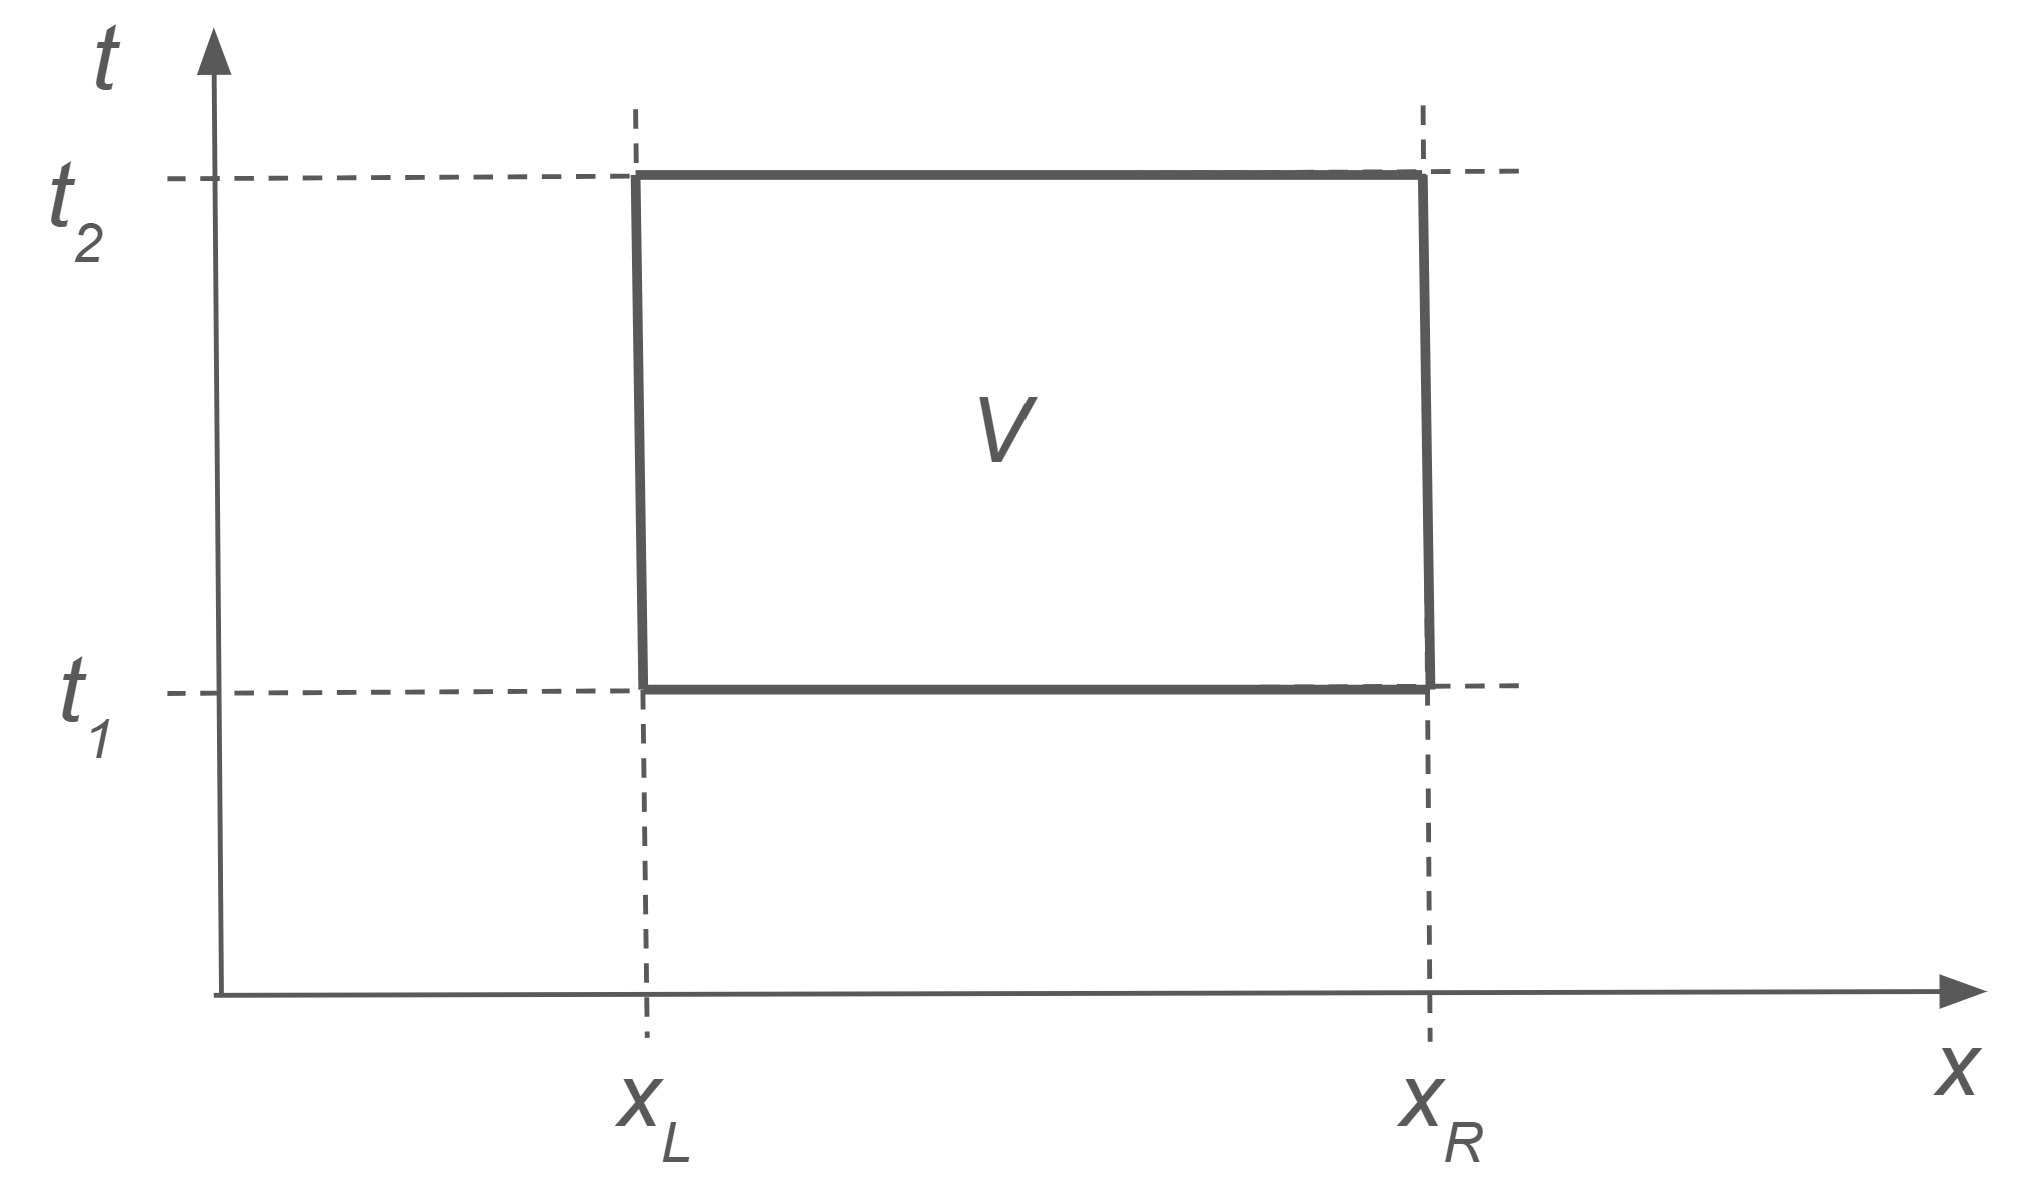
\includegraphics[width=0.5\textwidth]{C:/Users/Matteo/Shallow-Water-Equations/figs/Control_volume_1D.png}
    \caption{Illustration of a control volume $V$ in the $x,t$ plane. Illustration modified from~\cite{Toro2024}.}\label{fig:control_volume_1D}
\end{figure}
First we integrate the vector form of the SWE~\eqref{eq:vector_form_1D} over $x$ from $x_L$ to $x_R$ to obtain
\begin{align}\label{eq:derive_integral_form_1D}
    \int_{x_L}^{x_R} \mathbf{U}_t \text{ d}x + \int_{x_L}^{x_R} \mathbf{F(U)}_x \text{ d}x = \int_{x_L}^{x_R} \mathbf{S(U)} \text{ d}x.
\end{align}
Using the fundamental theorem of calculus, we get that 
\begin{align*}
    \int_{x_L}^{x_R} \mathbf{F}(\mathbf{U}) \text{ d}x = \mathbf{F}(\mathbf{U}(x_R, t)) - \mathbf{F}(\mathbf{U}(x_L, t)),
\end{align*}
which we insert in~\eqref{eq:derive_integral_form_1D}:
\begin{align}\label{eq:derive_integral_form_1D_2}
    \int_{x_L}^{x_R} \mathbf{U}_t \text{ d}x = \mathbf{F}(\mathbf{U}(x_L, t)) - \mathbf{F}(\mathbf{U}(x_R, t)) + \int_{x_L}^{x_R} \mathbf{S(U)} \text{ d}x.
\end{align}
Then we integrate~\eqref{eq:derive_integral_form_1D_2} over time from $t_1$ to $t_2$ to get
\begin{align*}
    \int_{t_1}^{t_2} \int_{x_L}^{x_R} \mathbf{U}_t \text{ d}x \text{d}t = \int_{t_1}^{t_2} \mathbf{F}(\mathbf{U}(x_L, t)) \text{ d}t - \int_{t_1}^{t_2} \mathbf{F}(\mathbf{U}(x_R, t)) \text{ d}t + \int_{t_1}^{t_2} \int_{x_L}^{x_R} \mathbf{S(U)} \text{ d}x \text{d}t.
\end{align*}
Rewriting the left hand side using the fundamental theorem of calculus, we get
\begin{align}\label{eq:integral_form_1D_final}
    \int_{x_L}^{x_R} \mathbf{U}(x, t_2) \text{ d}x =
    \int_{x_L}^{x_R}  \mathbf{U}(x, t_1) \text{ d}x + \int_{t_1}^{t_2} \mathbf{F}(\mathbf{U}(x_L, t)) \text{ d}t - \int_{t_1}^{t_2} \mathbf{F}(\mathbf{U}(x_R, t)) \text{ d}t + \int_{t_1}^{t_2} \int_{x_1}^{x_2} \mathbf{S(U)} \text{ d}x \text{d}t,
\end{align}
which is the integral form of the conservation laws for the SWE in 1D.
An alternative integral form of~\eqref{eq:vector_form_1D} is stated in~\cite{Toro2024}:
\begin{align}\label{eq:integral_form_1D_alternative}
    \frac{\text{d}}{\text{d}t} \int_{x_L}^{x_R} \mathbf{U}(x,t) \text{ d}x = \mathbf{F}(\mathbf{U}(x_L, t)) - \mathbf{F}(\mathbf{U}(x_R, t)) + \int_{x_L}^{x_R} \mathbf{S}(\mathbf{U}) \text{ d}x.
\end{align}
From~\eqref{eq:integral_form_1D_alternative} we get that the integral form of the homogeneous SWE in 1D is given by
\begin{align}\label{eq:integral_form_1D_homogeneous}
    \frac{\text{d}}{\text{d}t} \int_{x_L}^{x_R} \mathbf{U}(x,t) \text{ d}x = \mathbf{F}(\mathbf{U}(x_L, t)) - \mathbf{F}(\mathbf{U}(x_R, t)),
\end{align}
meaning that the rate of change of the integral over a domain is equal to the flux through the boundaries of the domain.


